\section{A aplicação Price Search}

\subsection{Proposta}
A aplicação PriceSearch foi pensado com o intuito de facilitar a pesquisa de preço de qualquer tipo de item existente no mercado, sejam eles eletrodomésticos, alimentos, utensílios, remédios, etc. Hoje em dia podemos encontrar diversos tipos de produtos em sites de grandes lojas, porém como existem várias cidades no Brasil que não possuem dessas grandes lojas, percebe-se que há uma grande dificuldade para saber em qual lugar tem tal item mais barato. Com isso, a ideia da aplicação é que as pessoas tenham acesso à um recurso para comparação de preço dos produtos dos estabelecimentos locais, a fim de ajudar as pessoas à economizar dinheiro. 

Outra ideia da aplicação é ajudar na busca de produtos, que antes não se sabia onde vendia. Com uma simples pesquisa, o usuário pode identificar facilmente o valor desse produto e onde encontrá-lo, através de um mapa que fornecerá a localização do estabelecimento contendo o seu endereço.

O intuito foi criar uma ferramenta simples, de fácil uso, e sendo ela multiplataformas, com o objetivo de agregar a quantidade máxima de usuários possíveis, para que todos possam usá-lo de maneira eficiente e rápida.

\subsection{Casos de Uso}
O diagrama de casos de uso da aplicação ilustra as ações de um usuário, que terá acesso às funções listadas, conforme a figura abaixo:

\begin{figure}[!htb]
\centering
\caption{Diagrama de Casos de Uso Price Search.}
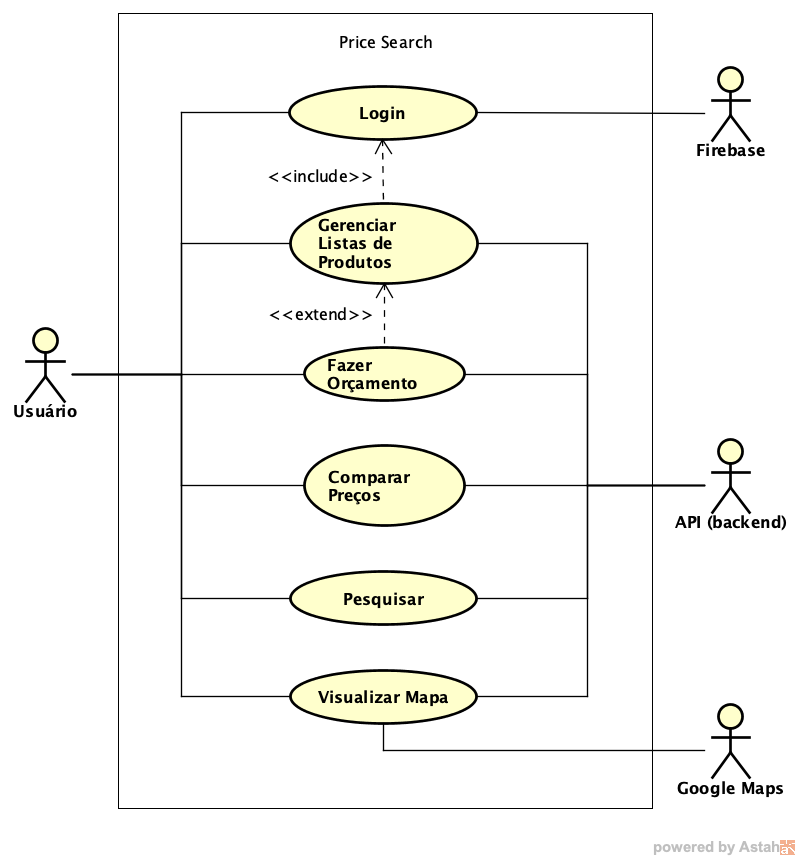
\includegraphics[width=\linewidth]{figuras/DiagramaCasosUsoPriceSearch.png}
{\footnotesize Fonte: Elaborado pelo autor.}
\end{figure}

\subsection{Caso de Uso 01: Login usuário}

O usuário inicia o login utilizando uma conta existente da Google, não sendo necessário preenchimento de nenhum tipo de dados. Feito isso, o assistente irá validar os dados do mesmo e o login será efetuado. Feito isso, nossa aplicação utilizará do ‘token’ fornecido pela conta do Google, para que possa ser salvo em nosso banco de dados para a sincronização das informações do usuário.

\subsection{Caso de Uso 02: Pesquisar}

A pesquisa será feita através dos nome de produtos, então o usuário poderá pesquisar por qualquer item, desde que o mesmo esteja no banco de dados. O sistema irá retornar todos os itens que tem o mesmo nome, no formato de uma lista. (perguntar se adiciona filtro).

\subsection{Caso de Uso 03: Gerenciar Lista de Compra}

O usuário poderá criar várias listas de compra como se fosse um carrinho de compras. Ao criar uma lista, o usuário poderá escolher um nome para ela; bem como escolher quais itens serão adicionados, e removê-los a qualquer momento; ou mesmo renomear a lista ou exclui-lá.

\subsection{Caso de Uso 04: Adicionar Favoritos}

Cada produto possui um botão para adicionar aos favoritos, que será uma aba na aplicação contendo a lista de todos os itens que foram salvos pelo usuário. Nesta lista ‘padrão’, o usuário também poderá adicionar e remover itens a qualquer momento.

\subsection{Caso de Uso 05: Visualizar Mapa}

O usuário terá acesso à um mapa que contém a localização de todos os estabelecimentos locais. Ao clicar nos estabelecimentos mostrados no mapa, irá ser fornecido informações sobre ele, como: nome e endereço.